\documentclass[twoside]{book}

% Packages required by doxygen
\usepackage{fixltx2e}
\usepackage{calc}
\usepackage{doxygen}
\usepackage{graphicx}
\usepackage[utf8]{inputenc}
\usepackage{makeidx}
\usepackage{multicol}
\usepackage{multirow}
\PassOptionsToPackage{warn}{textcomp}
\usepackage{textcomp}
\usepackage[nointegrals]{wasysym}
\usepackage[table]{xcolor}

% Font selection
\usepackage[T1]{fontenc}
\usepackage{mathptmx}
\usepackage[scaled=.90]{helvet}
\usepackage{courier}
\usepackage{amssymb}
\usepackage{sectsty}
\renewcommand{\familydefault}{\sfdefault}
\allsectionsfont{%
  \fontseries{bc}\selectfont%
  \color{darkgray}%
}
\renewcommand{\DoxyLabelFont}{%
  \fontseries{bc}\selectfont%
  \color{darkgray}%
}
\newcommand{\+}{\discretionary{\mbox{\scriptsize$\hookleftarrow$}}{}{}}

% Page & text layout
\usepackage{geometry}
\geometry{%
  a4paper,%
  top=2.5cm,%
  bottom=2.5cm,%
  left=2.5cm,%
  right=2.5cm%
}
\tolerance=750
\hfuzz=15pt
\hbadness=750
\setlength{\emergencystretch}{15pt}
\setlength{\parindent}{0cm}
\setlength{\parskip}{0.2cm}
\makeatletter
\renewcommand{\paragraph}{%
  \@startsection{paragraph}{4}{0ex}{-1.0ex}{1.0ex}{%
    \normalfont\normalsize\bfseries\SS@parafont%
  }%
}
\renewcommand{\subparagraph}{%
  \@startsection{subparagraph}{5}{0ex}{-1.0ex}{1.0ex}{%
    \normalfont\normalsize\bfseries\SS@subparafont%
  }%
}
\makeatother

% Headers & footers
\usepackage{fancyhdr}
\pagestyle{fancyplain}
\fancyhead[LE]{\fancyplain{}{\bfseries\thepage}}
\fancyhead[CE]{\fancyplain{}{}}
\fancyhead[RE]{\fancyplain{}{\bfseries\leftmark}}
\fancyhead[LO]{\fancyplain{}{\bfseries\rightmark}}
\fancyhead[CO]{\fancyplain{}{}}
\fancyhead[RO]{\fancyplain{}{\bfseries\thepage}}
\fancyfoot[LE]{\fancyplain{}{}}
\fancyfoot[CE]{\fancyplain{}{}}
\fancyfoot[RE]{\fancyplain{}{\bfseries\scriptsize Generated on Mon Dec 1 2014 22\+:49\+:08 for My Project by Doxygen }}
\fancyfoot[LO]{\fancyplain{}{\bfseries\scriptsize Generated on Mon Dec 1 2014 22\+:49\+:08 for My Project by Doxygen }}
\fancyfoot[CO]{\fancyplain{}{}}
\fancyfoot[RO]{\fancyplain{}{}}
\renewcommand{\footrulewidth}{0.4pt}
\renewcommand{\chaptermark}[1]{%
  \markboth{#1}{}%
}
\renewcommand{\sectionmark}[1]{%
  \markright{\thesection\ #1}%
}

% Indices & bibliography
\usepackage{natbib}
\usepackage[titles]{tocloft}
\setcounter{tocdepth}{3}
\setcounter{secnumdepth}{5}
\makeindex

% Hyperlinks (required, but should be loaded last)
\usepackage{ifpdf}
\ifpdf
  \usepackage[pdftex,pagebackref=true]{hyperref}
\else
  \usepackage[ps2pdf,pagebackref=true]{hyperref}
\fi
\hypersetup{%
  colorlinks=true,%
  linkcolor=blue,%
  citecolor=blue,%
  unicode%
}

% Custom commands
\newcommand{\clearemptydoublepage}{%
  \newpage{\pagestyle{empty}\cleardoublepage}%
}


%===== C O N T E N T S =====

\begin{document}

% Titlepage & ToC
\hypersetup{pageanchor=false,
             bookmarks=true,
             bookmarksnumbered=true,
             pdfencoding=unicode
            }
\pagenumbering{roman}
\begin{titlepage}
\vspace*{7cm}
\begin{center}%
{\Large My Project }\\
\vspace*{1cm}
{\large Generated by Doxygen 1.8.8}\\
\vspace*{0.5cm}
{\small Mon Dec 1 2014 22:49:08}\\
\end{center}
\end{titlepage}
\clearemptydoublepage
\tableofcontents
\clearemptydoublepage
\pagenumbering{arabic}
\hypersetup{pageanchor=true}

%--- Begin generated contents ---
\chapter{Hierarchical Index}
\section{Class Hierarchy}
This inheritance list is sorted roughly, but not completely, alphabetically\+:\begin{DoxyCompactList}
\item Abstract\+Table\+Model\begin{DoxyCompactList}
\item \contentsline{section}{movie.\+Movie\+Data\+Base}{\pageref{classmovie_1_1_movie_data_base}}{}
\end{DoxyCompactList}
\item J\+Frame\begin{DoxyCompactList}
\item \contentsline{section}{movie.\+Movie\+Frame}{\pageref{classmovie_1_1_movie_frame}}{}
\end{DoxyCompactList}
\item Serializable\begin{DoxyCompactList}
\item \contentsline{section}{movie.\+Movie}{\pageref{classmovie_1_1_movie}}{}
\end{DoxyCompactList}
\end{DoxyCompactList}

\chapter{Class Index}
\section{Class List}
Here are the classes, structs, unions and interfaces with brief descriptions\+:\begin{DoxyCompactList}
\item\contentsline{section}{\hyperlink{classmovie_1_1_movie}{movie.\+Movie} }{\pageref{classmovie_1_1_movie}}{}
\item\contentsline{section}{\hyperlink{classmovie_1_1_movie_data_base}{movie.\+Movie\+Data\+Base} }{\pageref{classmovie_1_1_movie_data_base}}{}
\item\contentsline{section}{\hyperlink{classmovie_1_1_movie_frame}{movie.\+Movie\+Frame} }{\pageref{classmovie_1_1_movie_frame}}{}
\end{DoxyCompactList}

\chapter{Class Documentation}
\hypertarget{classmovie_1_1_movie}{\section{movie.\+Movie Class Reference}
\label{classmovie_1_1_movie}\index{movie.\+Movie@{movie.\+Movie}}
}
Inheritance diagram for movie.\+Movie\+:\begin{figure}[H]
\begin{center}
\leavevmode
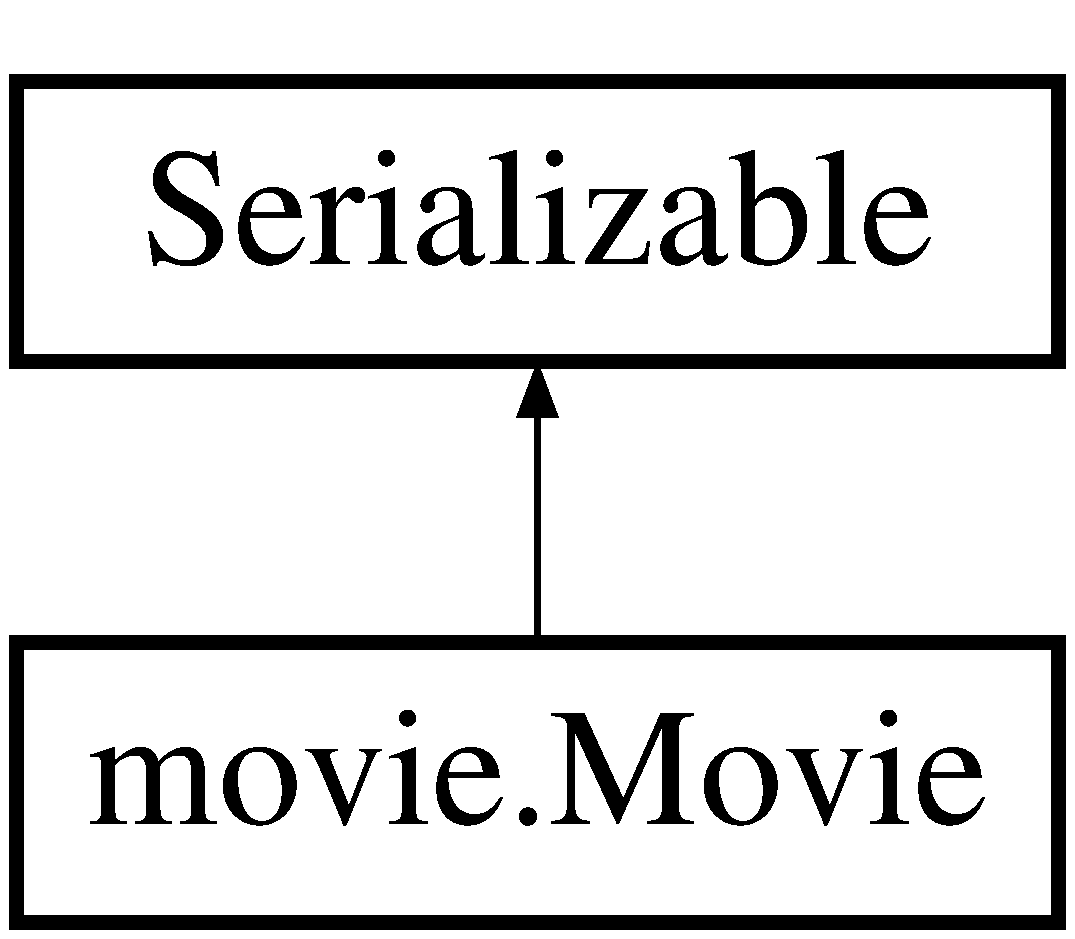
\includegraphics[height=2.000000cm]{classmovie_1_1_movie}
\end{center}
\end{figure}
\subsection*{Public Member Functions}
\begin{DoxyCompactItemize}
\item 
\hypertarget{classmovie_1_1_movie_a15bc1b3b3cefe583fbf221c46d905f3c}{{\bfseries Movie} (String title, String director, String premier, int length)}\label{classmovie_1_1_movie_a15bc1b3b3cefe583fbf221c46d905f3c}

\item 
String \hyperlink{classmovie_1_1_movie_a66c229e225f28090330e60d84ba3dc4a}{get\+Title} ()
\item 
int \hyperlink{classmovie_1_1_movie_a6cd818653c32498f1591f1f079fb0d0f}{get\+Length} ()
\item 
String \hyperlink{classmovie_1_1_movie_a0739ed120451a8bd3056620daba4c835}{get\+Premier} ()
\item 
String \hyperlink{classmovie_1_1_movie_afba9adf7eb86afd41c1db118fad5dbc9}{get\+Director} ()
\item 
boolean \hyperlink{classmovie_1_1_movie_a510c92052800fcf24d4951e85327bdb2}{is\+Marked} ()
\item 
void \hyperlink{classmovie_1_1_movie_a377992d8564030d8290c857973c9ba48}{set\+Marked} (boolean value)
\item 
boolean \hyperlink{classmovie_1_1_movie_a6b308eb2b1a64136b4127a1739129d81}{is\+Found} ()
\item 
void \hyperlink{classmovie_1_1_movie_ab58c507829f42de41b2540bb071333d8}{set\+Found} (boolean value)
\end{DoxyCompactItemize}


\subsection{Detailed Description}
Ez az oszt�ly t�rolja egy film adatait. Megval�s�tja a Serializable interf�szt, hogy ki lehessen menteni f�jlba az adatb�zihoz hozz�adott filmeket. 

\subsection{Member Function Documentation}
\hypertarget{classmovie_1_1_movie_afba9adf7eb86afd41c1db118fad5dbc9}{\index{movie\+::\+Movie@{movie\+::\+Movie}!get\+Director@{get\+Director}}
\index{get\+Director@{get\+Director}!movie\+::\+Movie@{movie\+::\+Movie}}
\subsubsection[{get\+Director}]{\setlength{\rightskip}{0pt plus 5cm}String movie.\+Movie.\+get\+Director (
\begin{DoxyParamCaption}
{}
\end{DoxyParamCaption}
)}}\label{classmovie_1_1_movie_afba9adf7eb86afd41c1db118fad5dbc9}
a film rendez�j�nek lek�rdez�se \begin{DoxyReturn}{Returns}
-\/ a film rendez�je 
\end{DoxyReturn}
\hypertarget{classmovie_1_1_movie_a6cd818653c32498f1591f1f079fb0d0f}{\index{movie\+::\+Movie@{movie\+::\+Movie}!get\+Length@{get\+Length}}
\index{get\+Length@{get\+Length}!movie\+::\+Movie@{movie\+::\+Movie}}
\subsubsection[{get\+Length}]{\setlength{\rightskip}{0pt plus 5cm}int movie.\+Movie.\+get\+Length (
\begin{DoxyParamCaption}
{}
\end{DoxyParamCaption}
)}}\label{classmovie_1_1_movie_a6cd818653c32498f1591f1f079fb0d0f}
a film hossz�nak lek�rdez�se \begin{DoxyReturn}{Returns}
-\/ a film hossza percekben 
\end{DoxyReturn}
\hypertarget{classmovie_1_1_movie_a0739ed120451a8bd3056620daba4c835}{\index{movie\+::\+Movie@{movie\+::\+Movie}!get\+Premier@{get\+Premier}}
\index{get\+Premier@{get\+Premier}!movie\+::\+Movie@{movie\+::\+Movie}}
\subsubsection[{get\+Premier}]{\setlength{\rightskip}{0pt plus 5cm}String movie.\+Movie.\+get\+Premier (
\begin{DoxyParamCaption}
{}
\end{DoxyParamCaption}
)}}\label{classmovie_1_1_movie_a0739ed120451a8bd3056620daba4c835}
a film premier�nek lek�rdez�se \begin{DoxyReturn}{Returns}
-\/ a film premier�nek d�tuma 
\end{DoxyReturn}
\hypertarget{classmovie_1_1_movie_a66c229e225f28090330e60d84ba3dc4a}{\index{movie\+::\+Movie@{movie\+::\+Movie}!get\+Title@{get\+Title}}
\index{get\+Title@{get\+Title}!movie\+::\+Movie@{movie\+::\+Movie}}
\subsubsection[{get\+Title}]{\setlength{\rightskip}{0pt plus 5cm}String movie.\+Movie.\+get\+Title (
\begin{DoxyParamCaption}
{}
\end{DoxyParamCaption}
)}}\label{classmovie_1_1_movie_a66c229e225f28090330e60d84ba3dc4a}
a film c�m�nek lek�rdez�se \begin{DoxyReturn}{Returns}
-\/ a film c�me 
\end{DoxyReturn}
\hypertarget{classmovie_1_1_movie_a6b308eb2b1a64136b4127a1739129d81}{\index{movie\+::\+Movie@{movie\+::\+Movie}!is\+Found@{is\+Found}}
\index{is\+Found@{is\+Found}!movie\+::\+Movie@{movie\+::\+Movie}}
\subsubsection[{is\+Found}]{\setlength{\rightskip}{0pt plus 5cm}boolean movie.\+Movie.\+is\+Found (
\begin{DoxyParamCaption}
{}
\end{DoxyParamCaption}
)}}\label{classmovie_1_1_movie_a6b308eb2b1a64136b4127a1739129d81}
a found �rt�k�nek lek�rdez�se \begin{DoxyReturn}{Returns}
-\/ true, ha megfelel a keres�si felt�teleknek, false, ha nem 
\end{DoxyReturn}
\hypertarget{classmovie_1_1_movie_a510c92052800fcf24d4951e85327bdb2}{\index{movie\+::\+Movie@{movie\+::\+Movie}!is\+Marked@{is\+Marked}}
\index{is\+Marked@{is\+Marked}!movie\+::\+Movie@{movie\+::\+Movie}}
\subsubsection[{is\+Marked}]{\setlength{\rightskip}{0pt plus 5cm}boolean movie.\+Movie.\+is\+Marked (
\begin{DoxyParamCaption}
{}
\end{DoxyParamCaption}
)}}\label{classmovie_1_1_movie_a510c92052800fcf24d4951e85327bdb2}
annak lek�rdez�se, hogy ki van-\/e jel�lve az adott film \begin{DoxyReturn}{Returns}
-\/ true, ha ki van jel�lve, false, ha nincs 
\end{DoxyReturn}
\hypertarget{classmovie_1_1_movie_ab58c507829f42de41b2540bb071333d8}{\index{movie\+::\+Movie@{movie\+::\+Movie}!set\+Found@{set\+Found}}
\index{set\+Found@{set\+Found}!movie\+::\+Movie@{movie\+::\+Movie}}
\subsubsection[{set\+Found}]{\setlength{\rightskip}{0pt plus 5cm}void movie.\+Movie.\+set\+Found (
\begin{DoxyParamCaption}
\item[{boolean}]{value}
\end{DoxyParamCaption}
)}}\label{classmovie_1_1_movie_ab58c507829f42de41b2540bb071333d8}
a found be�ll�t�sa 
\begin{DoxyParams}{Parameters}
{\em value} & -\/ az �rt�k, amire be�ll�tjuk \\
\hline
\end{DoxyParams}
\hypertarget{classmovie_1_1_movie_a377992d8564030d8290c857973c9ba48}{\index{movie\+::\+Movie@{movie\+::\+Movie}!set\+Marked@{set\+Marked}}
\index{set\+Marked@{set\+Marked}!movie\+::\+Movie@{movie\+::\+Movie}}
\subsubsection[{set\+Marked}]{\setlength{\rightskip}{0pt plus 5cm}void movie.\+Movie.\+set\+Marked (
\begin{DoxyParamCaption}
\item[{boolean}]{value}
\end{DoxyParamCaption}
)}}\label{classmovie_1_1_movie_a377992d8564030d8290c857973c9ba48}
a kijel�l�s be�ll�t�sa 
\begin{DoxyParams}{Parameters}
{\em value} & -\/ true vagy false, amire �ll�tani szeretn�nk a marked �rt�k�t \\
\hline
\end{DoxyParams}


The documentation for this class was generated from the following file\+:\begin{DoxyCompactItemize}
\item 
Movie.\+java\end{DoxyCompactItemize}

\hypertarget{classmovie_1_1_movie_data_base}{\section{movie.\+Movie\+Data\+Base Class Reference}
\label{classmovie_1_1_movie_data_base}\index{movie.\+Movie\+Data\+Base@{movie.\+Movie\+Data\+Base}}
}
Inheritance diagram for movie.\+Movie\+Data\+Base\+:\begin{figure}[H]
\begin{center}
\leavevmode
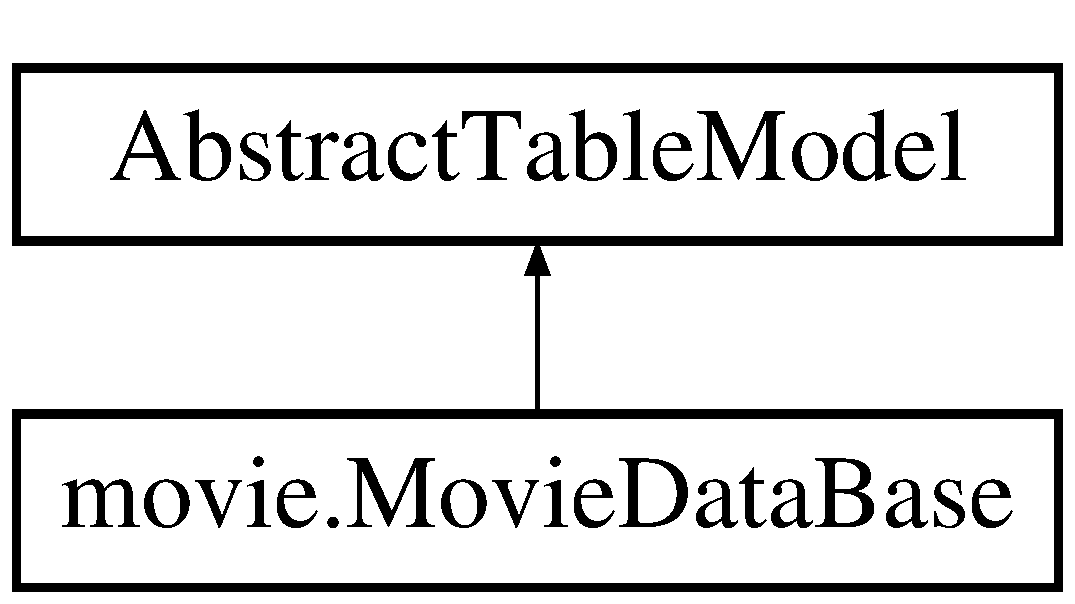
\includegraphics[height=2.000000cm]{classmovie_1_1_movie_data_base}
\end{center}
\end{figure}
\subsection*{Public Member Functions}
\begin{DoxyCompactItemize}
\item 
int \hyperlink{classmovie_1_1_movie_data_base_a35218c1a7743272e9a5780883ef31f8b}{get\+Row\+Count} ()
\item 
int \hyperlink{classmovie_1_1_movie_data_base_a2fa30de5e9bffd889c62617df9716b11}{get\+Column\+Count} ()
\item 
Object \hyperlink{classmovie_1_1_movie_data_base_a6f7ccc69b424c217cbeda6178495175c}{get\+Value\+At} (int row\+Index, int column\+Index)
\item 
String \hyperlink{classmovie_1_1_movie_data_base_a83038799f558bd8682bc531bcb9c8d95}{get\+Column\+Name} (int index)
\item 
Class$<$?$>$ \hyperlink{classmovie_1_1_movie_data_base_abf570a9f4b3f9c25a3977967f5b4c8d5}{get\+Column\+Class} (int index)
\item 
boolean \hyperlink{classmovie_1_1_movie_data_base_adec405f1fab1154a0d9064f877336f66}{is\+Cell\+Editable} (int row, int column)
\item 
void \hyperlink{classmovie_1_1_movie_data_base_a1b56aa6f04407b25b20991bfa0b55c8a}{set\+Value\+At} (Object value, int row, int column)
\item 
void \hyperlink{classmovie_1_1_movie_data_base_a05eb229b577536a71dd4831b9122cbe3}{add\+Movie} (\hyperlink{classmovie_1_1_movie}{Movie} m)
\item 
void \hyperlink{classmovie_1_1_movie_data_base_a48917199cfa02b6d8a26facdf77a22ee}{delete} ()
\item 
void \hyperlink{classmovie_1_1_movie_data_base_ae61245563faad4751e6a8fd1d6c9c780}{delete} (String option, String thing)
\item 
void \hyperlink{classmovie_1_1_movie_data_base_a4b04593497847c01cbd40c8a94af15b0}{search\+If} (String option, String thing)
\end{DoxyCompactItemize}


\subsection{Detailed Description}
Ez az oszt�ly alkotja az adatb�zist. Itt vannak elt�rolva a filmek adatai �s a hozz�juk kapcsol�d� met�dusok is ebben az oszt�lyban vannak defini�lva. Az oszt�ly megval�s�tja az Abstract\+Table\+Model interf�szt, hogy a t�bl�zat �t tudja venni az adatokat. 

\subsection{Member Function Documentation}
\hypertarget{classmovie_1_1_movie_data_base_a05eb229b577536a71dd4831b9122cbe3}{\index{movie\+::\+Movie\+Data\+Base@{movie\+::\+Movie\+Data\+Base}!add\+Movie@{add\+Movie}}
\index{add\+Movie@{add\+Movie}!movie\+::\+Movie\+Data\+Base@{movie\+::\+Movie\+Data\+Base}}
\subsubsection[{add\+Movie}]{\setlength{\rightskip}{0pt plus 5cm}void movie.\+Movie\+Data\+Base.\+add\+Movie (
\begin{DoxyParamCaption}
\item[{{\bf Movie}}]{m}
\end{DoxyParamCaption}
)}}\label{classmovie_1_1_movie_data_base_a05eb229b577536a71dd4831b9122cbe3}
egy film hozz�ad�sa az adatb�zishoz. ha m�r benne van az adatb�zisban, nem adjuk hozz� 
\begin{DoxyParams}{Parameters}
{\em m} & -\/ az adatb�zishoz hozz�adand� film \\
\hline
\end{DoxyParams}
\hypertarget{classmovie_1_1_movie_data_base_a48917199cfa02b6d8a26facdf77a22ee}{\index{movie\+::\+Movie\+Data\+Base@{movie\+::\+Movie\+Data\+Base}!delete@{delete}}
\index{delete@{delete}!movie\+::\+Movie\+Data\+Base@{movie\+::\+Movie\+Data\+Base}}
\subsubsection[{delete}]{\setlength{\rightskip}{0pt plus 5cm}void movie.\+Movie\+Data\+Base.\+delete (
\begin{DoxyParamCaption}
{}
\end{DoxyParamCaption}
)}}\label{classmovie_1_1_movie_data_base_a48917199cfa02b6d8a26facdf77a22ee}
a kijel�lt filmek t�rl�se az adatb�zisb�l \hypertarget{classmovie_1_1_movie_data_base_ae61245563faad4751e6a8fd1d6c9c780}{\index{movie\+::\+Movie\+Data\+Base@{movie\+::\+Movie\+Data\+Base}!delete@{delete}}
\index{delete@{delete}!movie\+::\+Movie\+Data\+Base@{movie\+::\+Movie\+Data\+Base}}
\subsubsection[{delete}]{\setlength{\rightskip}{0pt plus 5cm}void movie.\+Movie\+Data\+Base.\+delete (
\begin{DoxyParamCaption}
\item[{String}]{option, }
\item[{String}]{thing}
\end{DoxyParamCaption}
)}}\label{classmovie_1_1_movie_data_base_ae61245563faad4751e6a8fd1d6c9c780}
adott tulajdons�ggal rendelkez� filmek t�rl�se az adatb�zisb�l 
\begin{DoxyParams}{Parameters}
{\em option} & -\/ szempont, ami alapj�n t�r�lni akarunk filmeket \\
\hline
{\em thing} & -\/ ha az adott attrib�tuma a filmnek egyezik ezzel a sztringgel, vagy integerrel, akkor t�r�lj�k \\
\hline
\end{DoxyParams}
\hypertarget{classmovie_1_1_movie_data_base_abf570a9f4b3f9c25a3977967f5b4c8d5}{\index{movie\+::\+Movie\+Data\+Base@{movie\+::\+Movie\+Data\+Base}!get\+Column\+Class@{get\+Column\+Class}}
\index{get\+Column\+Class@{get\+Column\+Class}!movie\+::\+Movie\+Data\+Base@{movie\+::\+Movie\+Data\+Base}}
\subsubsection[{get\+Column\+Class}]{\setlength{\rightskip}{0pt plus 5cm}Class$<$?$>$ movie.\+Movie\+Data\+Base.\+get\+Column\+Class (
\begin{DoxyParamCaption}
\item[{int}]{index}
\end{DoxyParamCaption}
)}}\label{classmovie_1_1_movie_data_base_abf570a9f4b3f9c25a3977967f5b4c8d5}
az adatok megjelen�t�se a megfelel� form�tumban 
\begin{DoxyParams}{Parameters}
{\em index} & -\/ oszlopindex \\
\hline
\end{DoxyParams}
\begin{DoxyReturn}{Returns}
-\/ a megfelel� t�pus 
\end{DoxyReturn}
\hypertarget{classmovie_1_1_movie_data_base_a2fa30de5e9bffd889c62617df9716b11}{\index{movie\+::\+Movie\+Data\+Base@{movie\+::\+Movie\+Data\+Base}!get\+Column\+Count@{get\+Column\+Count}}
\index{get\+Column\+Count@{get\+Column\+Count}!movie\+::\+Movie\+Data\+Base@{movie\+::\+Movie\+Data\+Base}}
\subsubsection[{get\+Column\+Count}]{\setlength{\rightskip}{0pt plus 5cm}int movie.\+Movie\+Data\+Base.\+get\+Column\+Count (
\begin{DoxyParamCaption}
{}
\end{DoxyParamCaption}
)}}\label{classmovie_1_1_movie_data_base_a2fa30de5e9bffd889c62617df9716b11}
a t�bl�zathoz sz�ks�ges oszlopok sz�ma \begin{DoxyReturn}{Returns}
-\/ az oszlopok sz�ma, itt\+: 6, mert 6 oszlopunk lesz 
\end{DoxyReturn}
\hypertarget{classmovie_1_1_movie_data_base_a83038799f558bd8682bc531bcb9c8d95}{\index{movie\+::\+Movie\+Data\+Base@{movie\+::\+Movie\+Data\+Base}!get\+Column\+Name@{get\+Column\+Name}}
\index{get\+Column\+Name@{get\+Column\+Name}!movie\+::\+Movie\+Data\+Base@{movie\+::\+Movie\+Data\+Base}}
\subsubsection[{get\+Column\+Name}]{\setlength{\rightskip}{0pt plus 5cm}String movie.\+Movie\+Data\+Base.\+get\+Column\+Name (
\begin{DoxyParamCaption}
\item[{int}]{index}
\end{DoxyParamCaption}
)}}\label{classmovie_1_1_movie_data_base_a83038799f558bd8682bc531bcb9c8d95}
a fejl�cek be�ll�t�sa 
\begin{DoxyParams}{Parameters}
{\em index} & -\/ oszlopindex \\
\hline
\end{DoxyParams}
\begin{DoxyReturn}{Returns}
-\/ a megfelel� oszlop fejl�c�nek neve 
\end{DoxyReturn}
\hypertarget{classmovie_1_1_movie_data_base_a35218c1a7743272e9a5780883ef31f8b}{\index{movie\+::\+Movie\+Data\+Base@{movie\+::\+Movie\+Data\+Base}!get\+Row\+Count@{get\+Row\+Count}}
\index{get\+Row\+Count@{get\+Row\+Count}!movie\+::\+Movie\+Data\+Base@{movie\+::\+Movie\+Data\+Base}}
\subsubsection[{get\+Row\+Count}]{\setlength{\rightskip}{0pt plus 5cm}int movie.\+Movie\+Data\+Base.\+get\+Row\+Count (
\begin{DoxyParamCaption}
{}
\end{DoxyParamCaption}
)}}\label{classmovie_1_1_movie_data_base_a35218c1a7743272e9a5780883ef31f8b}
a t�bl�zathoz sz�ks�ges sorok sz�ma \begin{DoxyReturn}{Returns}
-\/ sorok sz�ma 
\end{DoxyReturn}
\hypertarget{classmovie_1_1_movie_data_base_a6f7ccc69b424c217cbeda6178495175c}{\index{movie\+::\+Movie\+Data\+Base@{movie\+::\+Movie\+Data\+Base}!get\+Value\+At@{get\+Value\+At}}
\index{get\+Value\+At@{get\+Value\+At}!movie\+::\+Movie\+Data\+Base@{movie\+::\+Movie\+Data\+Base}}
\subsubsection[{get\+Value\+At}]{\setlength{\rightskip}{0pt plus 5cm}Object movie.\+Movie\+Data\+Base.\+get\+Value\+At (
\begin{DoxyParamCaption}
\item[{int}]{row\+Index, }
\item[{int}]{column\+Index}
\end{DoxyParamCaption}
)}}\label{classmovie_1_1_movie_data_base_a6f7ccc69b424c217cbeda6178495175c}
a t�bl�zat cell�inak �rt�kei 
\begin{DoxyParams}{Parameters}
{\em row\+Index} & -\/ sorindex \\
\hline
{\em column\+Index} & -\/ oszlopindex \\
\hline
\end{DoxyParams}
\begin{DoxyReturn}{Returns}
-\/ az adott cella megfelel� tartalma 
\end{DoxyReturn}
\hypertarget{classmovie_1_1_movie_data_base_adec405f1fab1154a0d9064f877336f66}{\index{movie\+::\+Movie\+Data\+Base@{movie\+::\+Movie\+Data\+Base}!is\+Cell\+Editable@{is\+Cell\+Editable}}
\index{is\+Cell\+Editable@{is\+Cell\+Editable}!movie\+::\+Movie\+Data\+Base@{movie\+::\+Movie\+Data\+Base}}
\subsubsection[{is\+Cell\+Editable}]{\setlength{\rightskip}{0pt plus 5cm}boolean movie.\+Movie\+Data\+Base.\+is\+Cell\+Editable (
\begin{DoxyParamCaption}
\item[{int}]{row, }
\item[{int}]{column}
\end{DoxyParamCaption}
)}}\label{classmovie_1_1_movie_data_base_adec405f1fab1154a0d9064f877336f66}
az utols� (kiv�laszt�s) cell�t szerkeszthet�v� tessz�k 
\begin{DoxyParams}{Parameters}
{\em row} & -\/ sorindex (nincs r�s sz�ks�g) \\
\hline
{\em column} & -\/ oszlopindex \\
\hline
\end{DoxyParams}
\begin{DoxyReturn}{Returns}
-\/ szerkeszthe�-\/e vagy nem 
\end{DoxyReturn}
\hypertarget{classmovie_1_1_movie_data_base_a4b04593497847c01cbd40c8a94af15b0}{\index{movie\+::\+Movie\+Data\+Base@{movie\+::\+Movie\+Data\+Base}!search\+If@{search\+If}}
\index{search\+If@{search\+If}!movie\+::\+Movie\+Data\+Base@{movie\+::\+Movie\+Data\+Base}}
\subsubsection[{search\+If}]{\setlength{\rightskip}{0pt plus 5cm}void movie.\+Movie\+Data\+Base.\+search\+If (
\begin{DoxyParamCaption}
\item[{String}]{option, }
\item[{String}]{thing}
\end{DoxyParamCaption}
)}}\label{classmovie_1_1_movie_data_base_a4b04593497847c01cbd40c8a94af15b0}
adott tulajdons�ggal rendelkez� filmek keres�se 
\begin{DoxyParams}{Parameters}
{\em option} & -\/ szempont, ami alapj�n keres�nk \\
\hline
{\em thing} & -\/ ha az adott attrib�tuma a filmnek egyezik ezzel a sztringgel, vagy integerrel, akkor a found attrib�tum�t truera �ll�tjuk \\
\hline
\end{DoxyParams}
\hypertarget{classmovie_1_1_movie_data_base_a1b56aa6f04407b25b20991bfa0b55c8a}{\index{movie\+::\+Movie\+Data\+Base@{movie\+::\+Movie\+Data\+Base}!set\+Value\+At@{set\+Value\+At}}
\index{set\+Value\+At@{set\+Value\+At}!movie\+::\+Movie\+Data\+Base@{movie\+::\+Movie\+Data\+Base}}
\subsubsection[{set\+Value\+At}]{\setlength{\rightskip}{0pt plus 5cm}void movie.\+Movie\+Data\+Base.\+set\+Value\+At (
\begin{DoxyParamCaption}
\item[{Object}]{value, }
\item[{int}]{row, }
\item[{int}]{column}
\end{DoxyParamCaption}
)}}\label{classmovie_1_1_movie_data_base_a1b56aa6f04407b25b20991bfa0b55c8a}
az �t�ll�tott elemet elmentj�k a list�ban 
\begin{DoxyParams}{Parameters}
{\em value} & -\/ az �rt�k amire �t�ll�tjuk \\
\hline
{\em row} & -\/ sorindex \\
\hline
{\em column} & -\/ oszlopindex \\
\hline
\end{DoxyParams}


The documentation for this class was generated from the following file\+:\begin{DoxyCompactItemize}
\item 
Movie\+Data\+Base.\+java\end{DoxyCompactItemize}

\hypertarget{classmovie_1_1_movie_frame}{\section{movie.\+Movie\+Frame Class Reference}
\label{classmovie_1_1_movie_frame}\index{movie.\+Movie\+Frame@{movie.\+Movie\+Frame}}
}
Inheritance diagram for movie.\+Movie\+Frame\+:\begin{figure}[H]
\begin{center}
\leavevmode
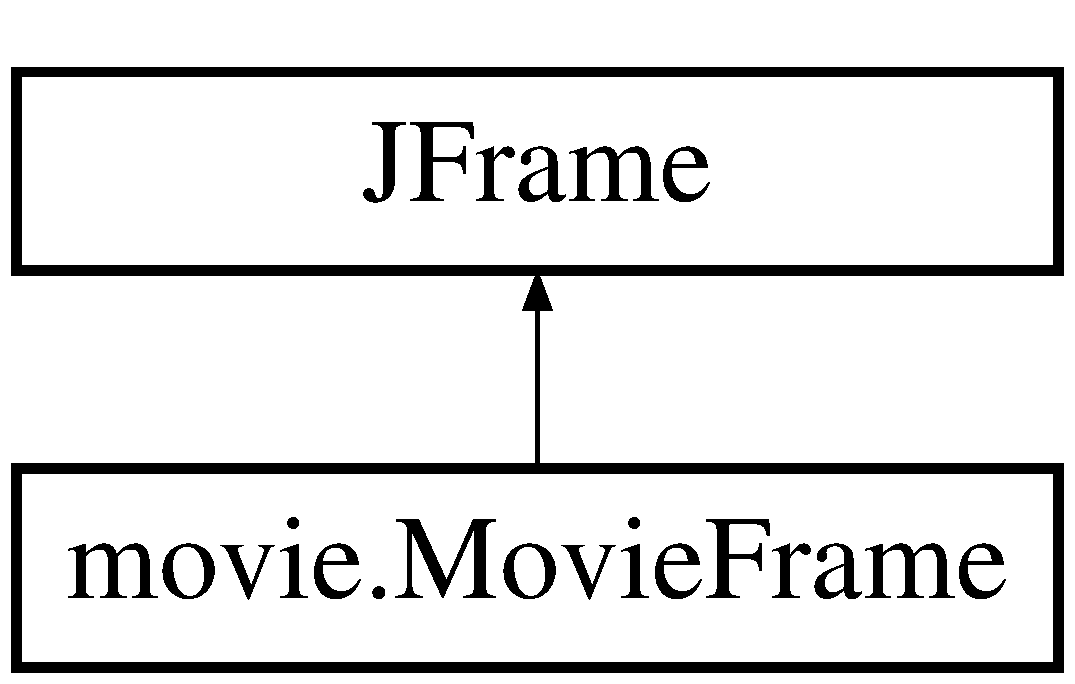
\includegraphics[height=2.000000cm]{classmovie_1_1_movie_frame}
\end{center}
\end{figure}


\subsection{Detailed Description}
Ez az oszt�ly a megjelen�t�s�rt felel�s, ez�rt �r�k�l a J\+Frame oszt�lyb�l. Az egyes komponensek (J\+Panel, J\+Button, J\+Table, J\+Text\+Field, J\+Combo\+Box) ebben az oszt�lyban vannak defini�lva �s az actionlistenereket is ebben az oszt�lyban kezelem. Ennek megfelel�en van az oszt�lyban egy My\+Action\+Listener bels� oszt�ly. 

The documentation for this class was generated from the following file\+:\begin{DoxyCompactItemize}
\item 
Movie\+Frame.\+java\end{DoxyCompactItemize}

%--- End generated contents ---

% Index
\newpage
\phantomsection
\addcontentsline{toc}{chapter}{Index}
\printindex

\end{document}
